
\documentclass{elsarticle}
\usepackage{booktabs}
\usepackage{multirow}
\usepackage[table,xcdraw]{xcolor}
\usepackage{multicol}
\usepackage{geometry}
\usepackage{setspace}
\usepackage{graphicx}
\usepackage{subcaption}
\usepackage{float}
\usepackage{caption}
\usepackage{natbib}
\usepackage [english]{babel}
\usepackage{blindtext}
\usepackage [autostyle, english = american]{csquotes}
\usepackage{etoolbox}
\usepackage{amsmath}
\usepackage{courier}

\apptocmd{\thebibliography}{\raggedright}{}{}
\MakeOuterQuote{"}

%\geometry{
%    top=3cm,
%    bottom=3cm,
%    left=3.5cm,
%    right=3.5cm,
%    headheight=14pt,
%}

%\captionsetup{font=footnotesize}
\begin{document}

\begin{frontmatter}

\title{Reservoir Computing with Complex Cellular Automata}
%\author{Neil Babson\\ \texttt{nbabson@pdx.edu}}
\author{Neil Babson} %\fnref{fn1}}}
\ead{nbabson@pdx.edu}

\author{Christof Teuscher}
\address{Portland State University, P.O.  Box 751, Portland, OR 97207-0751, 
   USA}
   
%\fntext[fn1]{   %\date{Portland State University -  \today}

%\begin{document}
%\maketitle

%\doublespacing

\begin{abstract}
Reservoir Computing is a computational framework in which a dynamical system, 
          known as the \textit{reservoir}, casts a temporal input signal to a 
          high-dimensional space, and a trainable \textit{readout layer} 
          creates the output signal by extracting salient features from the 
          reservoir.
A suitable reservoir  must possess the property of 
\textit{fading memory} in order to process inputs. The foundations of Reservoir Computing are the 
independently proposed Echo State Networks and Liquid State Machines, both of 
which use a randomly connected artificial recurrent neural network as the 
reservoir. Since the inception of the field, researchers have looked for ways 
to optimize the selection of reservoir construction parameters. Hierarchical 
reservoirs reimpose a degree of topological structure on reservoir connectivity 
by breaking the monolithic reservoir into loosely connected sub-reservoirs. The 
realization that dynamical systems besides neural networks could act as 
reservoirs has caused increasing interest in alternative reservoir substrates 
using biological, chemical, and physical dynamical systems. Several researchers 
have experimented with using the dynamical behavior of elementary cellular 
automaton rules as reservoirs. This research described in this paper expands 
this approach to cellular automaton with larger neighborhoods and/or more 
states, which are termed complex, as opposed to the elementary rules. Results 
show that some of these non-elementary cellular automaton rules outperform the 
best elementary rules at the standard benchmark 5-bit memory task, requiring 
half the reservoir size to produce comparable results.
\end{abstract}

\begin{keyword}
Reservoir computing \sep
Cellular automata

\end{keyword}

\end{frontmatter}


\begin{multicols}{2}
\section{Introduction}\label{introduction}
The small field of Cellular Automaton based Reservoir Computing (ReCA) has 
focused so far on the 256 elementary one-dimensional Cellular Automaton (CA) 
    rules which have two states and a neighborhood of size three. This work 
    expands ReCA to include one dimensional CA rules with larger neighborhoods 
    and more states.
    These rules that are not part of the set of one-dimensional elementary 
    rules will be referred to as \textit{complex} CA rules.  CA rule 
    performance is tested on the 5-bit memory task that is standard in ReCA 
    research. More expressive rules that outperform any of the elementary rules 
    require a smaller CA reservoir, reducing the amount of computation required 
    to train the output layer and to operate the reservoir.\par
    The remainder of the paper is organized as follows. Section 2 presents 
    background information on Reservoir Computing and Cellular Automata.  
    Section 3 outlines the ReCA system architecture used in the experiments.  
    The benchmark task used to evaluate the CA rules is described in Section 4.  
    Section 5 lists the complex CA experiments performed.  Sections 6 and 7 
    provide results and discussion. Future work is discussed in Section 8, and 
    Section 9 concludes the paper.   \section{Background}\label{background}
\subsection{Reservoir Computing}
Reservoir Computing (RC) is a relatively new approach to machine learning in 
which  the inner dynamics of a recurrently connected system, the 
\textit{reservoir}, are harnessed to cast temporal inputs into a 
high-dimensional space, enhancing their separability.  A \textit{readout layer} 
generates the output from a linear combination of the states of reservoir 
nodes. Figure \ref{reservoir_layout} shows the components of a reservoir 
computing system. The idea of reservoirs as a new type of architecture for 
Recurrent Neural Networks (RNNs) was proposed independently in 2001, under the 
name Echo State Networks (ESNS) \cite{jaeger2001echo}, and in 2002 as Liquid 
State Machines (LSMs) \cite{maass2002real}. The recurrent connections of a RNN 
cycle information back to the internal nodes, allowing them to possess 
\textit{state}, or memory, which makes them suitable for sequential tasks such 
as speech recognition. Unlike traditional neural networks, the internal weights 
between the nodes of the reservoir used in RC are not trained.  Only the 
weights to the output, or readout, layer are trained, providing a substantial 
reduction in the amount of computation required for learning. \par  A reservoir 
capable of representing the inputs in its internal dynamics can perform 
multiple computation tasks, even simultaneous tasks, by training different 
readout layers to extract the output. In both the original ESN and LSM 
reservoir design
nodes are connected at random, but as reservoirs found a growing number of 
successful applications, researchers examined alternate construction techniques 
\cite{lukovsevicius2007overview} and showed that many types of system besides 
RNNs produce effective reservoirs \cite{tanaka2018recent}.\par
    In order for a reservoir system to perform useful computation, it must 
    possess the \textit{echo-state property}, characterized by the term 
    \textit{fading memory}.  The system has the ability to remember (or echo) 
    inputs, but also forgets them over time. The \textit{echo-state property} 
    guarantees that the input driving the ESN will "wash out" the influence of 
    the random initial condition of the reservoir, causing it to react 
    predictably to inputs \cite{jaeger2001echo}. Dynamical systems operating at 
    the "edge of chaos" between ordered and disordered behavior are believed  
    to possess the highest computational power 
    \cite{langton1990computation}\cite{legenstein2007edge}.

\begin{figure}[H]
        \centering
            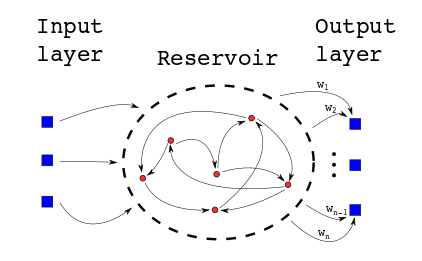
\includegraphics[width=0.4\textwidth]{Reservoir.png}
    \caption{Components of a reservoir computing system. Input is connected to 
        a subset of the reservoir nodes. Output is usually fully to the 
            reservoir. Only the outout weights $w_{i}$ for $i \in \{1, ..., 
            n\}$ are trained.} 
        
            \label{reservoir_layout}
            \end{figure}

\subsection{Cellular Automata}
Cellular Automata (CA) are dynamical systems composed of discrete cells 
arranged in a grid of arbitrary dimension (usually one, two or three 
        dimensional), where each cell is in one of a finite number of states.  
At each \textit{generation} the cells are synchronously updated to a new state 
according to the CA transition rule, which is a function of the cell's previous 
state and that of its neighboring cells. \par
The CA used in this paper are one-dimensional, which means that a cell's 
neighborhood is a row of an odd number of contiguous cells, centered on itself 
and including the immediate neighbors to the left and right.  Successive 
time steps are iterated downward to form a two-dimensional representation of the 
CA's evolution through time. The rule space of a CA depends on the size of the 
neighborhood, N, and the number of states, S. The cell states are numbered from 
0 to $S - 1$. The number of possible neighborhood states is $ S^N $ and each of 
these may be mapped by the transition rule to one of the S states, giving a 
total rule space of $ S^{S^N} $. A CA rule is used as a look-up table to apply 
the transition from each possible neighborhood state. Figure \ref{ca_rule} 
illustrates how a CA rule is applied.
\begin{figure}[H]
  \centering
    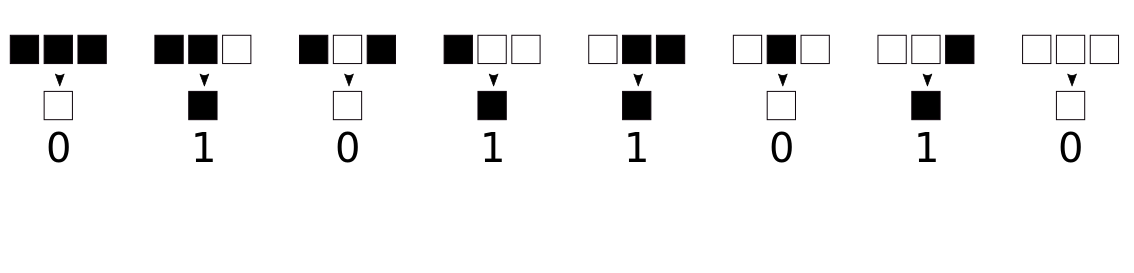
\includegraphics[width=0.4\textwidth]{Rule90.png}
    \caption{Elementary rule 90.}
        \label{ca_rule}
        \end{figure}

\par In his book \textit{A New Kind of Science} Wolfram systematically 
investigated the 256 one-dimensional rules with S = 2 and N = 3, which he named 
elementary cellular automata \cite{wolfram2002new}. An elementary rule's number 
is found by reading the rule as a binary number and converting it to base-10.  
Similarly, when $S = 3$ the rule number is determined by converting the lookup 
table from base-3 to base-10.
By convention, hexadecimal numbering is used for complex rules 
\cite{wuensche1999classifying}.

Wolfram also proposed a classification system based on the complexity of the 
emergent behavior of a CA rule. Class I CAs rapidly evolve to an homogeneous 
state from most  intial configurations.  Class II CAs evolve to a stable or 
simple periodic pattern.  Class III rules lead to chaotic behavior without 
stable structures.  In Class IV rules "edge of chaos" behavior can develop, 
       where localized structures can last for long periods, interacting with 
       each other in interesting and difficult to predict ways. An instance of 
       a Class IV rule, rule 110, has been proven to be Turing complete 
       \cite{cook2004universality}. Figure \ref{ca_complexity} shows examples 
       of the four classes.  \par

\begin{figure}[H]
  \centering
  \begin{subfigure}[]{0.2\linewidth}
    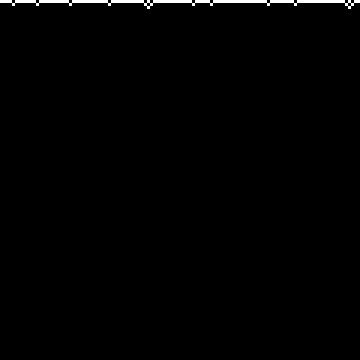
\includegraphics[width=\linewidth]{class1.png}
    \caption{}
  \end{subfigure}
  \begin{subfigure}[]{0.2\linewidth}
    
\includegraphics[width=\linewidth]{class2.png}
    \caption{}
  \end{subfigure}
  \begin{subfigure}[]{0.2\linewidth}
    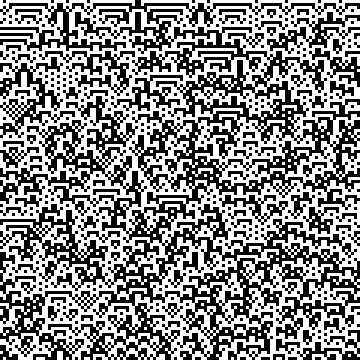
\includegraphics[width=\linewidth]{class3.png}
    \caption{}
  \end{subfigure}
  \begin{subfigure}[]{0.2\linewidth}
    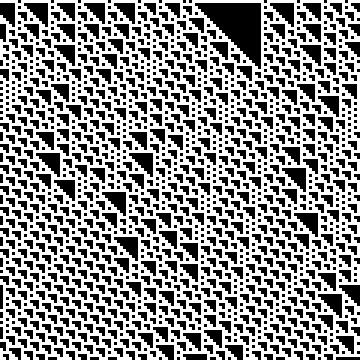
\includegraphics[width=\linewidth]{class4.png}
    \caption{}
  \end{subfigure}
  \caption{Wolfram's four classes of Cellular Automata rule represented by the 
      elementary rules. (a) Class I: Rule 215, (b) Class II: Rule 1, (c) Class 
          III: Rule 105, and (d) Class IV: Rule 193.}
  \label{ca_complexity}
  \end{figure}

\subsection{Previous Work}

The use of elementary cellular automaton rules for reservoir computing was 
   first proposed by Yilmaz in 2014, showing that the framework was capable of 
   solving memory tasks using orders of magnitude less computation than an ESN 
   \cite{yilmaz2014reservoir}. The name ReCA was introduced in 2016 by Margem 
   and Yilmaz \cite{margem2017experimental}. Bye investigated the perofrmance 
   of a ReCA system on the 30th order nonlinear autoregressive-moving-average 
   (NARMA) benchmark, the temporal bit parity and temporal bit density tasks, 
   as well as classification of vowel sound clips \cite{bye2016investigation}.  
      Non-uniform elementary CA reservoirs were used to solve the 5-bit memory 
      task by Nichele and Gunderson in 2017 \cite{nichele2017reservoir}. Also 
      in 2017 Nichele and Molund proposed a deep ReCA system using a 
      two-layered reservoir. Kleyko et al. demonstrated a ReCA system able 
      classify medical images with accuracy on par with traditional methods 
      \cite{kleyko2017modality}.
 





\section{Method}\label{method}
The ReCA system described in this section was implemented by the author in a 
C++ framework which can be found at https://github.com/nbabson/CAreservoir. The 
architecture of the framework is similar to that uesd in  
\cite{nichele2017deep} and \cite{bye2016investigation}.

\subsection{ReCA System Design}
The CA reservoir is made up of R sub-reservoirs which receive identical 
temporal input signals. This technique of duplicating the reservoir has been 
used since the original ReCA paper, and is found to be necessary for accurate 
results \cite{yilmaz2014reservoir}.
The leftmost cell of the first sub-reservoir is set to be the 
neighbor of the rightmost cell of the last sub-reservoir, creating a single 
circular CA.  Within each sub-reservoir a random mapping is generated between 
the elements of the input, of length $L_{n}$, and cells of the reservoir. The 
sub-reservoir size is known as the diffusion length, $L_{d}$, where $L_{n} < 
L_{d}$. The random mapping diffuses the inputs into the larger sub-reservoirs.  
\par The reservoir is initialized with all the cells in the same state, either 
0 for a two state CA, or the highest numbered state if $S > 2$. The initial 
input overwrites select cell states, according to the mapping. For applications 
with binary input, such the 5-bit memory benchmark, this is done by replacing 
the initial state of the $R \cdot L_{n}$ input cells with 0 or 1.  The 
reservoir processes the input by the application of the CA rule for I 
iterations, creating a CA reservoir of $R \cdot L_{d} \cdot (I + 1)$ cells.  
The initial $R \cdot L_{d} \cdot I$ cells are vectorized to provide the input 
to the readout layer, while the last $R \cdot L_{d}$ cells form the initial CA 
state for the next timestep, which is again selectively overwritten according 
to the input mapping. The rule is applied again, and the process repeats for 
each timestep of the input data.  \par  


Figure \ref{architecture} illustrates how the input is encoded into the 
reservoir and expanded by the CA rule to create the output vector.  The 
parameters S, N, R, $L_{d}$, and I can be set by command line arguments. An 
alternative scheme for combining the inputs with the reservoir, similar to that 
adopted by Yilmaz in \cite{yilmaz2015connectionist}, adds the input value to 
the current cell state according to equation \ref{eq:input}, where $s^{t+1}$ is 
the state of the input cell $s^t$ at the next timestep after combining with the 
input bit $i$.  Adding 1 to the resultant cell state ensures that every binary 
input affects the reservoir when $S > 2$.  This approach was found to produce 
inferior results and is not used in this paper.

              \begin{equation} \label{eq:input}
              s^{t+1} = (s^t + i + 1) \bmod S
              \end{equation}    


	      \begin{figure}[H]
        \centering
            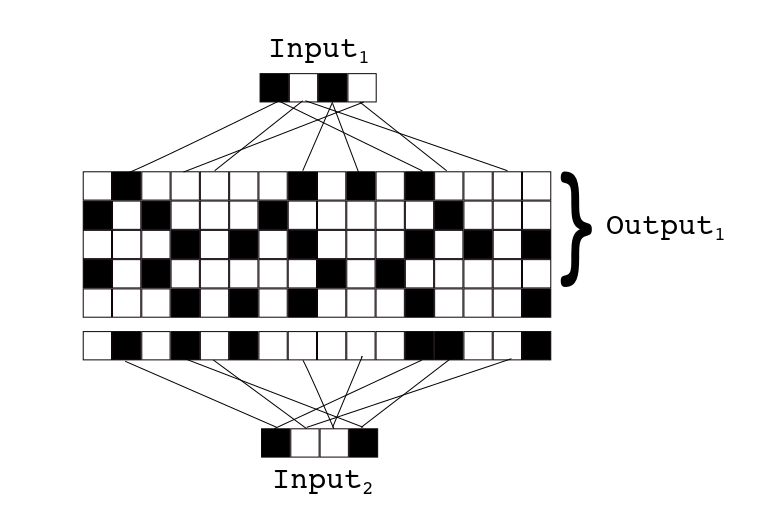
\includegraphics[width=0.4\textwidth]{Architecture.png}
    \caption{Mapping the input to the reservoir and generating the output.  
        $L_{n}$ = 4, $L_{d}$ = 8, R = 2, I = 4, Rule 90. Initially all the 
            cells of the reservoir are in the same state. At each timestep the 
            input is randomly mapped onto each of the R sub-reservoirs, 
                  overwriting the cell state. The CA rule is then applied I 
                      times. The last generation of the CA forms the initial 
                      state for the next timestep, which is again overwritten 
                      according to the input mapping. The rest of the CA is 
                      vectorized and sent to the output nodes. } 
        
            \label{architecture}
            \end{figure}

\subsection{Readout Layer}
The 5-bit memory task requires the network to predict three output bits per 
timestep.  Accordingly, the ReCA system that performs it has three output 
nodes.  The weight from identical locations of the CA created at each timestep 
are treated equally, and used to predict output by reflecting the system's 
response to inputs. The output weights from the $R \cdot L_{n} \cdot I$ ReCA 
cells to the readout nodes are set using a linear regression model. The outputs 
from all time steps, as well as the target values, are sent to the linear 
regression model all at once for fitting.  \par
After the weights are set, the task is run again and the system predicts the 
outputs. The real-valued output of the linear regression at the output nodes is 
binarized, with output smaller than 0.5 rounded to 0, and equal or greater to 
0.5 rounded to 1. \par The ReCA system uses two different linear regression 
implementations, the linreg package from the C++ AlgLib library, and the 
linear\_model.LinearRegression class from the Python scikit-learn library.  The 
two implementations produced equivalent results but the sci-kit functions ran 
faster, so sci-kit is used for the experiments in this paper. The system also 
allows the option of  using support vector machines (SVM) from the C++ Torch 
machine learning library as the classifier.  Stefano Nichele and Magnus 
Gunderson used SVM in their 2017 ReCA paper on non-uniform 
reservoirs\cite{nichele2017reservoir}.

\section{Benchmark Tests}\label{Benchmarks}
\subsection{Five Bit Memory Task}\label{5_bit}
The 5-bit memory task benchmark tests a network's long-short-term-memory 
capability, and has been shown to be difficult for recurrent neural networks, 
    including ESN \cite{hochreiter1997long}\cite{jaeger2012long}. All of the 
    literature on ReCA uses the 5-bit task benchmark, so it is an appropriate 
    first test of the capabilities of complex versus elementary CA reservoirs.  
    The task has four temporal binary input signals, $i_1, i_2, i_3,$ and 
    $i_4$, and three binary outputs, $o_1, o_2,$ and $o_3$.  During the
first five time steps of one run of the input sequence, the $i_1$ input is one 
of the 32 possible five digit binary numbers, while $i_2$ is always $(i_1 + 1) 
    mod 2$ (1 when $i_1 = 0$ and vice versa). This is the \textit{message} that 
    the system is supposed to remember. While the message is being input, $i_3 
    = i_4 = 0$.  \par  This is followed by a \textit{distractor period} of 
    $T_d$ timesteps.  Following convention in ReCA research, all tests in this 
    paper were done with $T_d = 200$.  On all time steps of the distractor 
    period except the last, $i_1 = i_2 = 0, i_3 = 1, $ and $i_4 = 0$. On the 
    last step of the distractor period, $i_4 = 1$, giving the cue signal that 
    it is time for the system to reproduce the pattern. Up until this point the 
    expected output is $o_1 = o_2 = 0 $ and $0_3 = 1$. For the remaining five 
    time steps of the run the output bits should be the same as the 
    \textit{message}, i.e.  the same as the first three input bits during the 
    first five time steps.  While the message is repeated, the inputs are the 
    same as during the distractor period, $o_1 = o_2 = o_4 = 0$ and $o_3 = 1$.  
    Table \ref{table:5_bit} illustrates one run of the 5-bit task. \par
    This series of $T_d + 10$ time steps is a single run of the test and is 
    repeated for each of the 32 possible message inputs. To pass the 5-bit task 
    the trained system must correctly predict the output bits for all steps of 
    the task. With $T_d = 200$, that is $210 \cdot 32 \cdot 3 = 20,160$ accurate 
    predictions.

% Please add the following required packages to your document preamble:
% \usepackage{multirow}
% \usepackage[table,xcdraw]{xcolor}
% If you use beamer only pass "xcolor=table" option, i.e.
\iffalse
\begin{table*}[t]  \centering
\small
\begin{tabular}{|c|l|l|l|l|l|l|l|l}
\cline{1-8}
\multicolumn{1}{|l|}{Time step} & \multicolumn{4}{l|}{Input} & \multicolumn{3}{l|}{Output} & \cellcolor[HTML]{FFFFFF}{\color[HTML]{333333} } \\ \hline
1 & \cellcolor[HTML]{96FFFB}1 & \cellcolor[HTML]{96FFFB}0 & 0 & 0 & 0 & 0 & 1 & \multicolumn{1}{l|}{} \\ \cline{1-8}
2 & \cellcolor[HTML]{96FFFB}0 & \cellcolor[HTML]{96FFFB}1 & 0 & 0 & 0 & 0 & 1 & \multicolumn{1}{l|}{} \\ \cline{1-8}
3 & \cellcolor[HTML]{96FFFB}0 & \cellcolor[HTML]{96FFFB}1 & 0 & 0 & 0 & 0 & 1 & \multicolumn{1}{l|}{} \\ \cline{1-8}
4 & \cellcolor[HTML]{96FFFB}0 & \cellcolor[HTML]{96FFFB}1 & 0 & 0 & 0 & 0 & 1 & \multicolumn{1}{l|}{} \\ \cline{1-8}
5 & \cellcolor[HTML]{96FFFB}1 & \cellcolor[HTML]{96FFFB}0 & 0 & 0 & 0 & 0 & 1 & \multicolumn{1}{l|}{\multirow{-5}{*}{\begin{tabular}[c]{@{}l@{}}Input\\ message\end{tabular}}} \\ \hline
6 & 0 & 0 & 1 & 0 & 0 & 0 & 1 & \multicolumn{1}{l|}{} \\ \cline{1-8}
... & 0 & 0 & 1 & 0 & 0 & 0 & 1 & \multicolumn{1}{l|}{} \\ \cline{1-8}
204 & 0 & 0 & 1 & 0 & 0 & 0 & 1 & \multicolumn{1}{l|}{\multirow{-3}{*}{\begin{tabular}[c]{@{}l@{}}Distractor\\ period\end{tabular}}} \\ \hline
205 & 0 & 0 & 0 & 1 & 0 & 0 & 1 & \multicolumn{1}{l|}{Cue Signal} \\ \hline
206 & 0 & 0 & 1 & 0 & \cellcolor[HTML]{96FFFB}1 & \cellcolor[HTML]{96FFFB}0 & 0 & \multicolumn{1}{l|}{} \\ \cline{1-8}
207 & 0 & 0 & 1 & 0 & \cellcolor[HTML]{96FFFB}0 & \cellcolor[HTML]{96FFFB}1 & 0 & \multicolumn{1}{l|}{} \\ \cline{1-8}
208 & 0 & 0 & 1 & 0 & \cellcolor[HTML]{96FFFB}0 & \cellcolor[HTML]{96FFFB}1 & 0 & \multicolumn{1}{l|}{} \\ \cline{1-8}
209 & 0 & 0 & 1 & 0 & \cellcolor[HTML]{96FFFB}0 & \cellcolor[HTML]{96FFFB}1 & 0 & \multicolumn{1}{l|}{} \\ \cline{1-8}
210 & 0 & 0 & 1 & 0 & \cellcolor[HTML]{96FFFB}1 & \cellcolor[HTML]{96FFFB}0 & 0 & \multicolumn{1}{l|}{\multirow{-5}{*}{\begin{tabular}[c]{@{}l@{}}Repeat\\ Message\end{tabular}}} \\ \hline
\end{tabular}
\caption{Run 17 of 32 of the 5-bit memory task.}
\label{table:5_bit}
\end{table*}
\fi

\begin{table}[H]
\centering
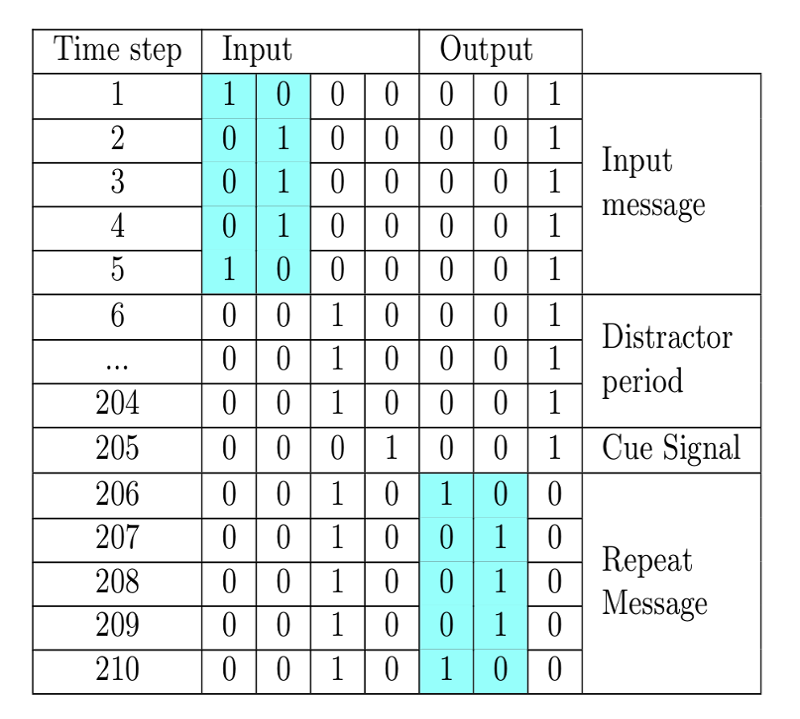
\includegraphics[width=0.4\textwidth]{5bit.png}
\caption{Run 17 of 32 of the 5-bit memory task.}
\label{table:5_bit}
\end{table}


\subsection{Temporal Density and Temporal Parity}
For both the temporal density and the temporal parity classification tasks the 
    reservoir receives a single input stream of bits. The reservoirs were 
    tested on both tasks simultaneously using the same input stream.  
    \section{Experiments}\label{experiment}
\subsection{5-Bit Memory Task}
In order to establish a baseline for the performance of the complex CA rules on 
    the 5-bit memory task, the ReCA framework was tested on a selection of 
    elementary CA rules which were found to be the most successful at the task 
    in previous work\cite{yilmaz2014reservoir}\cite{bye2016investigation}. With 
    I = 4 and R = 8, only four elementary rules were able to achieve zero error 
    on the 5-bit task. These four rules are equivalent, being either mirror 
    images of each other and/or having their states reversed.\par Increasing 
    the reservoir size by adding sub-reservoirs or applying the rule more times 
    improved accuracy, but came at a cost of increased processing time required 
    to perform the linear regression.  Table \ref{table:elementary} shows the 
    results for the most promising elementary rules at different combinations 
    of I and R.  Table \ref{table:time} gives average times to train and test 
    elementary CA reservoirs of different sizes. The results obtained here were 
    somewhat worse for the smaller reservoir of (I,R) = (4,8) than in previous 
    work using a similar system design  
    \cite{bye2016investigation}\cite{yilmaz2014reservoir}\cite{nichele2017reservoir}.  
    \par Finding more effective rules among complex CA enables the task to be 
    reliably completed with a smaller reservoir than is required by an 
    elementary CA, thereby reducing the amount of computation required. All of 
    the experiments described in this section were performed with (I,R) = (4,8) 
    and $L_{d} = 40$.  Only rules that passed the 5-bit task on their first run 
    were saved for further testing. Since none of the elementary CA rules were 
    able to pass the benchmark as much as 10\% of the time, this means that 
    many rules which are capable of outperforming any of the elementary rules 
    were rejected. 


\begin{table}[H] \centering
\begin{tabular}{|l|l|l|l|}
\hline
\textbf{Rule} & \textbf{(I,R)=(4,8)} & \textbf{(8,8)} & \textbf{(4,12)} \\ 
\hline
60 & 9 & 99 & 92 \\ \hline
90 & 0 & 22 & 2  \\ \hline
102 & 9 & 99 & 86 \\ \hline
153 & 6 & 99 & 87 \\ \hline
195 & 6 & 99 & 92 \\ \hline
210 & 6 & 12 & 66 \\ \hline
\end{tabular}
\caption{Successful trials out of 100 for elementary CA rules on the 5-bit 
    task.}
\label{table:elementary}
\end{table}

\begin{table}[H] \centering
\begin{tabular}{|l|l|}
\hline
\textbf{(I,R)} & \textbf{Time} \\ \hline
(4,8) & 19 s \\ \hline
(4,12) & 33 s \\ \hline
(8,8) & 57 s \\ \hline
\end{tabular}
\caption{Time in seconds to train and test a reservoir using elementary rule 60 
    on the 5-bit task for different values of I and R. Times are averages of 
        five test runs.}
\label{table:time}
\end{table}

  
\subsubsection{Three State CA Reservoir}
One dimensional CAs with three states and a neighborhood of three have a 
transition function specified by a lookup table 27 digits long. The rule space 
is $3^27 \approx 7.6 \cdot 10^12$. A stochastic search of the space randomly 
generated rules to test on the 5-bit memory task. As the most computationally 
intensive part of the search is performing the linear regression on the 
reservoirs, class I and class II rules, whose behavior is believed to be too 
simple to support computation, are removed. The CAs are first evolved according 
to their rule without any inputs beyond a random initial configuration. Rules 
for CA that settle into a uniform or oscillating state in the first 100 
generations, as well as those that merely shift to the left or right, are 
removed from consideration.\par
The remaining rules are tested on the 5-bit memory task.  Those that succeed 
without any inaccurate predictions are saved for further testing.  These are 
then scored on 100 runs of the 5-bit task.  Out of a thousand runs, rules that 
passed the benchmark were found 2.0\% of the time, and 17.6\% of the randomly 
generated rules were discarded as class I or II.
    
\subsubsection{Neighborhood Five CA Reservoir}
Two state neighborhood five rules have a rule space of $2^32 \approx 4.3 \cdot 
    10^9$. As with three state neighborhood three rules, this space was 
    searched stochastically, with class I and class II rules ignored. Rules for 
    reservoirs that pass the 5-bit memory task are saved and tested on 100 
    further runs of the benchmark. Of 1000 runs, 2.2\% of randomly generated 
    rules passed the benchmark, and 16.2\% of the rules were rejected before 
    testing for being class I or class II.
\subsubsection{Population Density Rules}
Population density transition rules are a function of a cell's state and the 
    count of how many cells are in each state $s \in S$ among its neighbors. 
    For (S,N) = (2,5), these are a left-right symmetrical subset of the two 
    state neighborhood five rules. The transition function lookup table is 10 
    digits long, and each of the 1024 rules were investigated. Those exhibiting 
    class I or class II behavior were rejected while the rest were tested on 
    the 5-bit memory task. Nine rules passed the benchmark. Those that passed 
    were saved and tested on the benchmark 100 times.

  \subsubsection{Evolving Complex CA Rules}
Complex CA with more than three states have a vast rule space. For (S,N) = 
    (3,4) and (S,N) = (3,5) the number of possible CA rules are $\approx 3.4 \cdot 
    10^38$ and $\approx 2.4 \cdot 10^87$ respectively. These spaces are not 
    amenable to a stochastic search for rules able to perform the 5-bit memory 
    task.  Hundreds of randomly generated rules failed to produce any that were 
    successful. Almost all of these reservoirs mapped every input to the most 
    frequently occurring expected output for each output layer node. This is 
    because the vast majority of these rules are class III, too chaotic to 
    allow stable structures too persist and therefore unable to support 
    computation.\par
In order to reduce the chaoticity, a genetic algorithm (GA) was used to evolve 
rules more likely to have class III behavior. The very chaotic rules found by 
randomly generating a CA with $S > 3$ tend to have small contiguous regions in 
their two dimensional representation of development in time, resembling 
television static.  The GA fitness function selects for rules more likely to 
have class IV behavior by maximizing the size of these contiguous regions, 
     which allows for the possibility of developing stable localized 
     structures. \par The GA algorithm starts with a randomly generated 
     population of 32 rules. At each epoch the rule is applied for 200 
     iterations to an initial random configuration of 400 cells.  The fitness 
     of each individual is evaluated using a "smallest-largest" rule.  The 
     largest contiguous region of cells belonging to the same state, adjacent 
     horizontally or vertically, is identified for each state $s \in S$. The 
     fitness assigned to the rule is equal to the size of the smallest of these 
     largest connected areas. Using the area for the state whose contiguous 
     region is smallest ensures that all the states contribute to the dynamic 
     behavior of the CA rule and prevents the tendency for the GA to evolve 
     toward a uniform class I behavior. \par The least fit half of the 
     population are discarded and replaced by the next generation of offspring.  
     The fit half of the population forms eight pairs that each produce two new 
     rules by separating at a randomly chosen location and recombining, as seen 
     in Fig. \ref{GA}. Each new rule receives a single random mutation changing 
     one digit of its rule. Evolution continues for 200 generations or until 
     the fitness of the best individual equals or exceeds 200, which rarely 
     takes more than 150 generations.  \par Both the mating and the mutation 
     portion of the algorithm were found to be necessary, with either one 
     removed evolution happens much more slowly if at all. The fitness goal of 
     at least 200, for both four state and five state rules, was chosen 
     empirically as the point where the evolved rules were making the least 
     incorrect predictions when given the 5-bit task. \par
     The evolved four state rules passed the benchmark 2.5\% of the time and 
     the five state rules passed 1.1\%. Many more missed less than 10 
     predictions, which was not observed to happen with unevolved rules.




\begin{figure}[H]
  \centering
    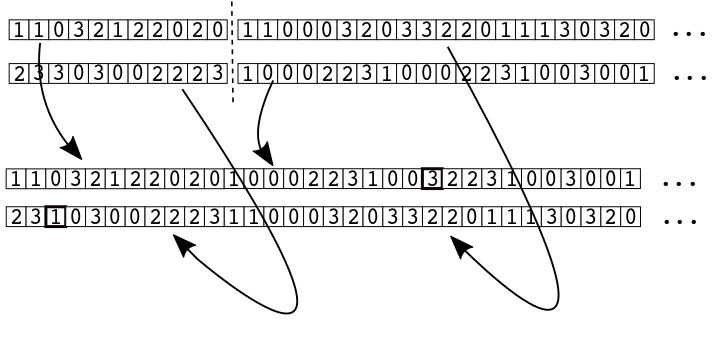
\includegraphics[width=\linewidth]{GA.png}
  \caption{Two rules produce a pair of children by splitting at a randomly 
      chosen point and recombining. Each child receives a single random 
          mutation.}
  \label{GA}
  \end{figure}

\subsubsection{Non-Uniform Reservoir}
A non-uniform CA is one in which the cells don't all implement the same rule.  
    The ReCA framework used here implements a parallel non-uniform CA in which 
    the reservoir is split in half into two sub-reservoirs  using different 
    rules.  The cells at the boundaries between  the two sub-reservoirs 
    consider their neighbors in the other sub-reservoir the same as those in 
    their own sub-reservoir in the application of the rule. This allows 
    information to to flow between the two regions. Previous work has shown 
    that certain combinations of elementary rules in a parallel ReCA perform 
    better than either of the rules individually at the 5-bit memory task while 
    other combinations impeded performance\cite{nichele2017reservoir}.  \par In 
    this work combinations of complex rules were tested together to show that 
    complementary rule combinations exist for the different types of complex CA 
    rules investigated.  
    
\subsection{Temporal Density and Temporal Parity}

\section{Results}\label{results}
%\subsection{Elementary CA Results}
From each of the types of rules that were investigated, the six most successful 
rules at performing the benchmark task using reservoirs with parameters (I, R, 
        $L_{d}$) = (4, 8, 40) were selected for testing with smaller  
reservoirs. In the absence of a naming convention for the complex rules, these 
were given labels. The best performing rules and their labels are seen in Table
\ref{table:rules}. \par

\begin{table*}[!htb] \centering
\small
\begin{tabular}{|p{2cm}|l|}
\hline
\multicolumn{2}{|l|}{\textbf{Three State Rules (S,N) = (3,3)}} \\ \hline
%$S3_{1}$ &  022001212222022121202001201 \\ \hline
$S3_{1}$ &  212aa02ad02\\ \hline
%$S3_{2}$ &  212001112001100202012121112 \\ \hline
$S3_{2}$ &  5ec2484e083\\ \hline
%$S3_{3}$ &  110211111111012011002221221 \\ \hline
$S3_{3}$ &  34be5823dc1\\ \hline
%$S3_{4}$ &  112220001122200202101120022 \\ \hline
$S3_{4}$ &   3d337739e3f\\ \hline
%$S3_{5}$ &  120000111211201212122222020 \\ \hline
$S3_{5}$ &   3db9f53398b\\ \hline
%$S3_{6}$ &  210121202010220010012001002 \\ \hline
$S3_{6}$ &   58db54c1a35\\ \hline
\multicolumn{2}{|l|}{\textbf{Neighborhood Five Rules (S,N) = (2,5)}} \\ \hline
%$N5_{1}$ &  10011011100011011100011101100000 \\ \hline
$N5_{1}$ &   9b8dc760\\ \hline
%$N5_{2}$ &  00000000110011011101111101000000 \\ \hline
$N5_{2}$ &    cddf40\\ \hline
%$N5_{3}$ &  01110010010111111011001001000000 \\ \hline
$N5_{3}$ &   725fb240\\ \hline
%$N5_{4}$ &  11111101001110100110110100010010 \\ \hline
$N5_{4}$ &   fd3a6d12\\ \hline
%$N5_{5}$ &  01001111011100010110000101010100 \\ \hline
$N5_{5}$ &   4f716154\\ \hline
%$N5_{6}$ &  01110001111011100011101010101111 \\ \hline
$N5_{6}$ &   71ee3aaf\\ \hline
\multicolumn{2}{|l|}{\textbf{Density Rules (S,N) = (2,5)}} \\ \hline
%$D_{1}$ &  0100111011\\ \hline
$D_{1}$ &   13b \\ \hline
%$D_{2}$ &  1001010100\\ \hline
$D_{2}$ &   254 \\ \hline
%$D_{3}$ &  1011010000\\ \hline
$D_{3}$ &   2d0 \\ \hline
%$D_{4}$ &  1111001010\\ \hline
$D_{4}$ &   3ca \\ \hline
%$D_{5}$ &  1001110101\\ \hline
$D_{5}$ &   275 \\ \hline
%$D_{6}$ &  1010001101\\ \hline
$D_{6}$ &   28d \\ \hline
\multicolumn{2}{|l|}{\textbf{Four State Rules (S,N) = (3,3)}} \\ \hline
%$S4_{1}$ &  2321222211000231312322232311322030112313011100201322000131220020\\ 
$S4_{1}$ &   b9aa502ddbabb5e8c5b715087a01da08\\ \hline
%$S4_{2}$ &  3202120010220311333022122021303233302103221213012310122021121000\\ 
$S4_{2}$ &   e2604a35fca689cefc93a671b4689640 \\ \hline
%$S4_{3}$ &  0133030132200000320101302012232200212322332332000000130331110303\\ 
$S4_{3}$ &   1f31e800e11c86ba09bafbe00073d533\\ \hline
%$S4_{4}$ &  2330232310230333132321011123101333310111101120123322023101112201\\ 
$S4_{4}$ &   bcbb4b3f7b915b47fd154586fa2d15a1\\ \hline
%$S4_{5}$ &  1103233321313023211332211232000210133021222120002201022101311332\\ 
$S4_{5}$ &   53bf9dcb97e96e0247c9a980a1291d7e \\ \hline
%$S4_{6}$ &  1303200320121103303030201311010210331123101211201101121212023003\\
$S4_{6}$ &   73838653ccc875124f5b4658516662c3\\
\hline
\multicolumn{2}{|l|}{\textbf{Five State Rules (S,N) = (3,3)}} \\ \hline
 $S5_{1}$ & %  {\begin{tabular}[c]{@{}l@{}}
%1301443104221322240300230403103441002312212144030011314304232243323124040221\\ 
    %    4204330141121024304340424234410332033014231100030\ \end{tabular}} \\ 
    1871abdbbb1f751c5649ce2208abe0525e5e98543e527293d8fe32c1cbec8f9493da900dc 
    \\
    \hline
    $S5_{2}$ & %{\begin{tabular}[c]{@{}l@{}}
%1203233110034020231023234244243332104432100104440412333033104430212221401123
%    4302014024200311301004200203233323023204121113342\ \end{tabular}} \\ ff 
159b7bf409f219a835b7bbe69791bfa94432d737117268fff0b99044ac2ccbb513ca91456 \\
\hline
$S5_{3}$ & %{\begin{tabular}[c]{@{}l@{}}
%1400243030402041101342340202043101140340113112143144030220022044324410141400
%    1144040240413332111020130224434041240241032000030\ \end{tabular}}
1b4cca207dfd49a79d60a0f0a36fda79a911db434135e22cd79e6e04c69f086c7aab1712a
\\ \hline
$S5_{4}$  & %{\begin{tabular}[c]{@{}l@{}}
%1421333424244211231320221124334213323140314040030314242321304343413222403434
%    1443102441033314110213410404041140002414124400043\ \end{tabular}}
1ca6bafcb8cc14e379373cb798461269c4d81258cc28720c74f12dd39b8e48d5863e176a9
\\ \hline
$S5_{5}$ & %{\begin{tabular}[c]{@{}l@{}}
%3420313303232322101243344342044403031133414314300043124201312322441210243102
%    0012332434010222311113213123044310440203144333200\ \end{tabular}} 
3ac662317b4445a8e63b425645228e27bfc4a0a388497b03a0adede89e87685b12977008f
\\ \hline
$S5_{6}$ & %{\begin{tabular}[c]{@{}l@{}}
%0133104314321000400141320442032240002333312104040024401313033202213203300242
%    3234304312240443431412304141033301200200241442030\ \end{tabular}} 
53b86edcbce84369a1eeb58079725743b506f228e9459e488139f0763489461f3847c82a
\\ \hline
\end{tabular}
\caption{The six best rules from each of the categories of complex CA rule 
    investigated.}
\label{table:rules}
\end{table*}


The selected rules were then tested 100 times each with a range of the 
reservoir parameters I, R, and $L_{d}$.  The results can be seen in Table 
\ref{table:results}. 

\begin{table*}[!htb] \centering
\small
\begin{tabular}{|l|l|l|l|l|l|l|}
\hline
\textbf{Rule} & \textbf{(I,R,$L_{d}$)=(4,8,40)} & \textbf{(4,8,30)} & 
\textbf{(4,6,40)} & \textbf{(4,4,40)} & \textbf{(3,8,40)} & \textbf{(4,8,20)} 
\\ \hline
\multicolumn{7}{|l|}{\textbf{Elementary Rules (S,N) = (2,3)}} \\ \hline
60 & 9 & - & - & - & - & - \\ \hline
90 & 0 & - & - & - & - & - \\ \hline
102 & 9 & - & - & - & - & - \\ \hline
153 & 6 & - & - & - & - & - \\ \hline
195 & 6 & - & - & - & - & - \\ \hline
210 & 6 & - & - & - & - & - \\ \hline
\multicolumn{7}{|l|}{\textbf{Three State Rules (S,N) = (3,3)}} \\ \hline
$S3_{1}$ & 100 & 100 & 100 & 0 & 25 & 10 \\ \hline
$S3_{2}$ & 99 & 63 & 44 & 0 & 16 & 0 \\ \hline
$S3_{3}$ & 100 & 92 & 89 & 2 & 0 & 6 \\ \hline
$S3_{4}$ & 100 & 53 & 42 & 0 & 0 & 0 \\ \hline
$S3_{5}$ & 100 & 85 & 93 & 2 & 2 & 0 \\ \hline
$S3_{6}$ & 99 & 97 & 79 & 6 & 5 & 0 \\ \hline
\multicolumn{7}{|l|}{\textbf{Neighborhood Five Rules (S,N) = (2,5)}} \\ \hline
$N5_{1}$ & 97 & 83 & 61 & 0 & 0 & 0 \\ \hline
$N5_{2}$ & 99 & 92 & 60 & 0 & 0 & 2 \\ \hline
$N5_{3}$ & 99 & 98 & 69 & 0 & 88 & 2  \\ \hline
$N5_{4}$ & 95 & 75 & 59 & 0 & 0 & 0 \\ \hline
$N5_{5}$ & 95 & 87 & 26 & 0 & 0 & 0 \\ \hline
$N5_{6}$ & 93 & 49 & 46 & 35 & 38 & 0  \\ \hline
\multicolumn{7}{|l|}{\textbf{Density Rules (S,N) = (2,5)}} \\ \hline
$D_{1}$ & 68 & 47 & 23 & 0 & 1 & 0  \\ \hline
$D_{2}$ & 70 & 0 & 6 & 0 & 0 & 0 \\ \hline
$D_{3}$ & 94 & 62 & 63 & 0 & 0 & 20 \\ \hline
$D_{4}$ & 96 & 87 & 57 & 0 & 0 & 0 \\ \hline
$D_{5}$ & 99 & 17 & 35 & 0 & 25 & 0 \\ \hline
$D_{6}$ & 64 & 58 & 27 & 0 & 1 & 0 \\ \hline
\multicolumn{7}{|l|}{\textbf{Four State Rules (S,N) = (3,3)}} \\ \hline
$S4_{1}$ & 90 & 75 & 58 & 0 & 12  & 1 \\ \hline
$S4_{2}$ & 90 & 84 & 56 & 0 & 9 & 0  \\ \hline
$S4_{3}$ & 93 & 12 & 9 & 0 & 42 & 0 \\ \hline
$S4_{4}$ & 95 & 35 & 21 & 0 & 0 & 0 \\ \hline
$S4_{5}$ & 100 & 85 & 66 & 0 & 11 & 1 \\ \hline
$S4_{6}$ & 87 & 20 & 2 & 0 & 0 & 0 \\ \hline
\multicolumn{7}{|l|}{\textbf{Five State Rules (S,N) = (3,3)}} \\ \hline
$S5_{1}$ & 95 & 50 & 42 & 8 & 15 & 0 \\ \hline
$S5_{2}$ & 95 & 76 & 70 & 0 & 7 & 0 \\ \hline
$S5_{3}$ & 98 & 74 & 51 & 0 & 24 & 0 \\ \hline
$S5_{4}$ & 80 & 1 & 9 & 0 & 2 & 0 \\ \hline
$S5_{5}$ & 84 & 17 & 7 & 0 & 2 & 0 \\ \hline
$S5_{6}$ & 77 & 13 & 6 & 0 & 5 & 0 \\ \hline
\end{tabular}
\caption{Successful runs out of 100 on 5-bit task for elementary CA and five 
    types of complex CA rule.}
\label{table:results}
\end{table*}


\section{Discussion}\label{discussion}
While the best performing elementary rules required a reservoir of size $I \cdot R 
\cdot L_{d} = 8 \cdot 8 \cdot 40 = 2560$ cells in order to achieve 99\% success on the 
5-bit memory task, each of the five categories of complex CA rule investigated 
here produced a rule capable of achieving 99\% or 100\% success on a reservoir 
of half that size, $I \cdot R \cdot L_{d} = 4 \cdot 8 \cdot 40 = 1280$ cells. The best 
performing rules discovered were three state neighborhood three. One of these 
was able to produce 100\% correct results using a reservoir of size $I \cdot R \cdot 
L_{d} = 4 \cdot 6 \cdot 40 = 960$ cells. Only the neighborhood five population density 
rules were investigated exhaustively.  For the other rule categories continued 
searching would yield a virtually infinite number of similarly successful 
rules. \par Rule performance correlates broadly with reservoir size, but the 
ability of the ReCA system to  pass the benchmark falls at different rates 
depending on which of the reservoir parameters I, R, or $L_{d}$ is lowered. The 
30 complex rules average 91.7\% correct test runs on the 1280 cell reservoir.  
Reducing the reservoir size by 1/4 by lowering the diffusion length to 30 
caused the least performance degradation, with the average success rate at 
56.6\%. Reducing the reservoir size by cutting the number of sub-reservoirs 
from eight to six had a slightly larger effect on the average reservoir 
performance, which fell to 45.9\%.  Finally, when the reservoir size was 
reduced to 960 cells by lowering the number of iterations, I, from four to 
three, the average success rate was only 11.0\%, with 11 rules achieving zero 
correct runs, while a  couple of rules were  relatively resilient to the 
reduced iterations. When the reservoir size was halved from 1280 to 640  cells, 
        the majority of the complex rules were unable to to complete any 
            successful runs of the task, and the average success rate was only 
            1.9\%. \par An attempt was made to find pairs of rules that would 
            complement each other in a non-uniform reservoir, performing better 
            than either rule would alone, as has been shown to sometimes occur 
            with pairs of elementary rules \cite{nichele2017reservoir}. The six 
            rules of each complex rule type can form 75 combinations of 
            same-type rules each of which can be used as a non-uniform 
            reservoir for  any setting of the reservoir size parameters. Of 
            these possibilities, 20 combinations were tested with 100 runs of 
            the benchmark. Pairs of rules were selected that performed well 
            individually with the same reservoir parameters.  None of these 
            pairs performed better than the more successful of the two in a 
            uniform reservoir, 11 of the pairings performing significantly 
            worse than either rule tested alone. While it seems very likely 
            that complex CA non-uniform pairings exist which do work well 
            together, it remains an open question how common or rare they are.
 

\begin{figure}[H]
\centering
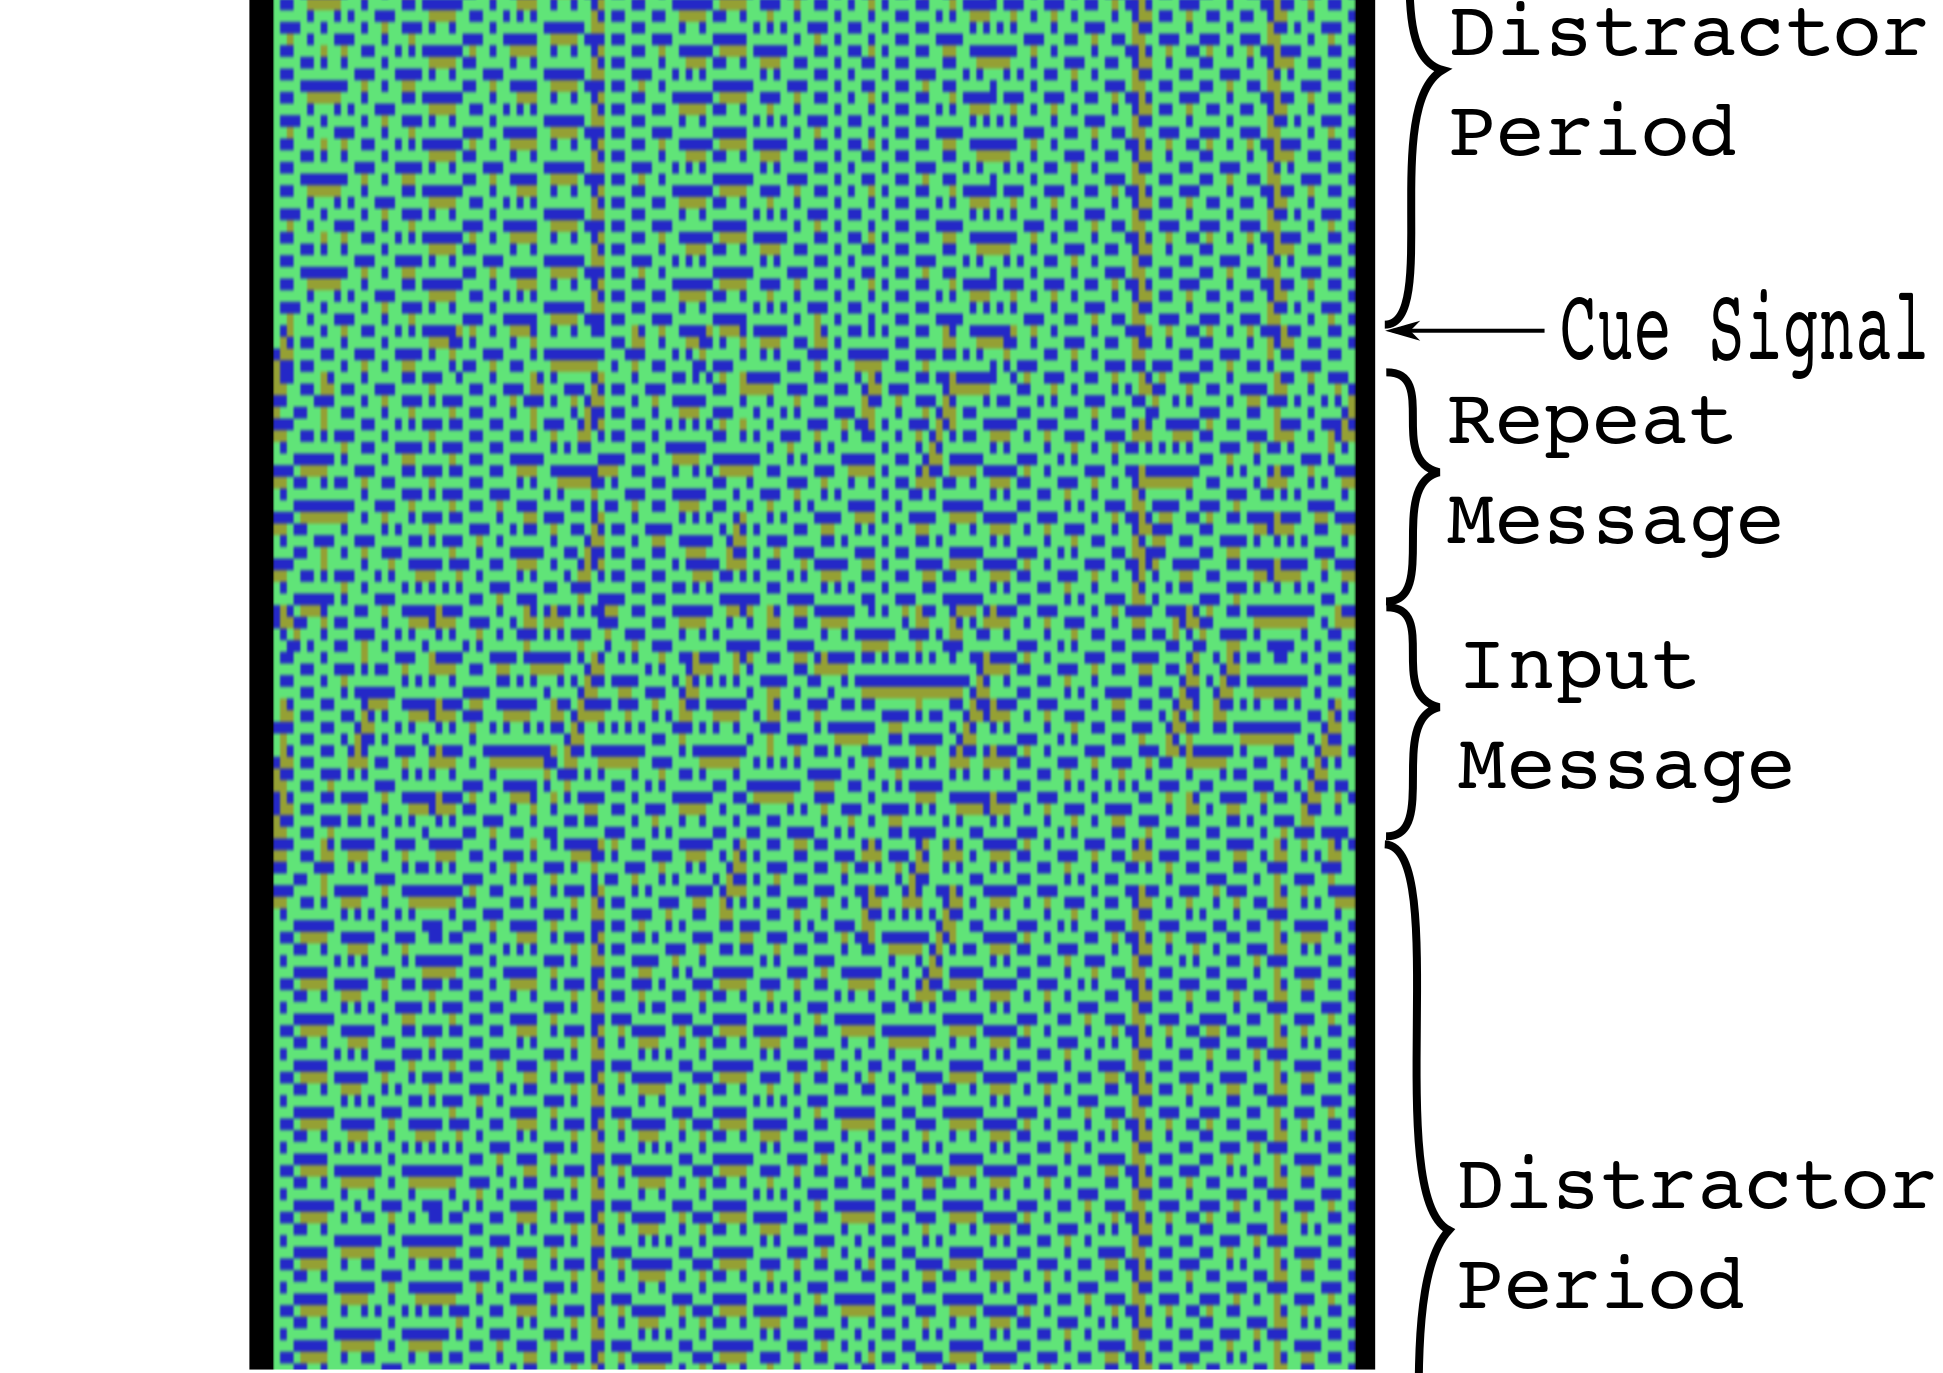
\includegraphics[width=0.4\textwidth]{RepeatMessage.png}
\caption{A segment of the history of a reservoir using rule $S3_{1}$ on the 
   5-bit task with I=4, R=8, and $D_{L}$=30. Each four horizontal lines is one 
      reservoir timestep. At the top of the image is the end of the distractor 
      period after the input message 00001. The reservoir has fallen into a 
      stable repeating pattern with a period of eight generations. After the 
      cue signal is received the reservoir "remembers" the message that was 
      encoded in the repeating pattern. After the next message 00010 is input 
      the reservoir quickly falls into another stable pattern that encodes the 
      new message.} 
        
\label{repeat}
\end{figure}

\iffalse

\section{Future Work}\label{future_work}
The next step in investigating complex CA rules for ReCA would be to measure 
the chaoticity of the most successful rules in comparison to the average, using 
measures such as Shannon entropy, Langton's $\lambda$ parameter, and the 
Lyapunov exponent. It would be interesting to see whether the successful rules 
do tend to cluster in an "edge of chaos" region of complexity, and whether this
is true for different benchmark tasks. \par Other fitness functions could be 
explored for evolving CA rules towards a desired chaoticity. The existence of 
an "edge of chaos" region of complexity densely populated with successful rules 
would mean that reservoir rules could be constructed with the requisite degree 
of complexity at lower computational cost and greater accuracy than being 
evolved.  \par Further examination of non-uniform complex ReCA reservoirs could 
apply different types of rules in parallel i.e.  rules with different 
neighborhood size or number of states.  Different types of rules may exhibit 
differing behaviors that in some circumstances synergistically combine in a 
beneficial manner.  Measurements of rule chaoticity might also be able to shed 
some light on why certain combinations are complementary. It is also possible 
that given one successful rule, techniques for constructing a complementary 
rule could be discovered.

\fi
\section{Conclusion}\label{conclusion}
A reservoir computing with cellular automata (ReCA) framework has been 
implemented which expands the field of ReCA research from the 256 elementary 
cellular automata rules to investigate rules with larger neighborhoods and more 
states, here called \textit{complex} CA rules. A genetic algorithm was used to 
reduce the chaoticity of the four state and five state rule space, in order to 
find \textit{edge of chaos} rules capable of computing the 5-bit memory task 
benchmark. \par The six best rules from each of five categories of complex rule 
were tested and shown to require half of the reservoir size as the most 
successful elementary rules to produce comparable results. This reduction in 
reservoir size equals a saving in power and time when operating the reservoirs.

\bibliographystyle{ieeetr}
\bibliography{CAReservoir}

\end{multicols}
\end{document}
